\documentclass[letterpaper, 10 pt, onecolumn]{ieeeconf}  

\IEEEoverridecommandlockouts                              % This command is only
                                                          % needed if you want to
                                                          % use the \thanks command


\usepackage{graphicx}
\usepackage{amsmath}
\usepackage{amssymb}
\usepackage{hyperref}

\title{\LARGE \bf Machine Learning Project Proposal: Solar Flare Forecasting}

\author{Dave Achyut$^{1}$ and J. Marcus Hughes$^{1, 2}$ and Mahesh Parab$^{1}$% <-this % stops a space
\thanks{$^{1}$Department of Computer Science, University of Colorado Boulder, Boulder, CO}%
\thanks{$^{2}$Marcus has support from domain experts Daniel Seaton, Robert Steenburgh, and Hazel Bain at the National Oceanic and Atmospheric Administration (NOAA), space weather and solar experts who are interested in this project for research and operations. They will guide the project with domain expertise.}
}

\begin{document}
\maketitle
\thispagestyle{empty}
\pagestyle{empty}

%%%%%%%%%%%%%%%%%%%%%%%%%%%%%%%%%%%%%%%%%%%%%%%%%%%%%%%%%%%%%%%%%%%%%%%%%%%%%%%%
\begin{abstract}
Solar flares can impact humans in many negative ways such as disrupting communications, harming astronauts, damaging electrical power grids. Our project will focus on forecasting the future brightness once one has begun. 

\end{abstract}

%%%%%%%%%%%%%%%%%%%%%%%%%%%%%%%%%%%%%%%%%%%%%%%%%%%%%%%%%%%%%%%%%%%%%%%%%%%%%%%%
\section{MOTIVATION AND BACKGROUND}
Solar flares are sudden releases of energy from the Sun with harmful effects such as disrupting electrical power grids, damaging satellites, and endangering astronauts. Many groups are working to forecast whether this will be a solar flare hours to days in the future, see \cite{bobra, guerra, yu, nishizuka}. That problem is very challenging. A smaller, interesting problem that has not been explored is predicting a flare's evolution on a shorter time scale of minutes to hours. During a flare, the observed brightness increases rapidly and then decreases as the flaring event ends as shown in Figure \ref{fig:example}. Our task is to forecast how bright a flare will be in the future after observing a portion of it in a given wavelength interval (referred to from here on as a passband). Predicting when and how bright a flare will peak will allow quicker response for space weather forecast centers and ultimately quicker alerts. Even more so, there are scientific questions that can be addressed by knowing how well we can predict (the stability of flaring regions), what information is most useful in prediction (insight on what the most important drivers in flaring are), and when the regressor fails (understanding of potentially different types of flares).

\begin{figure}[h!]
    \centering
    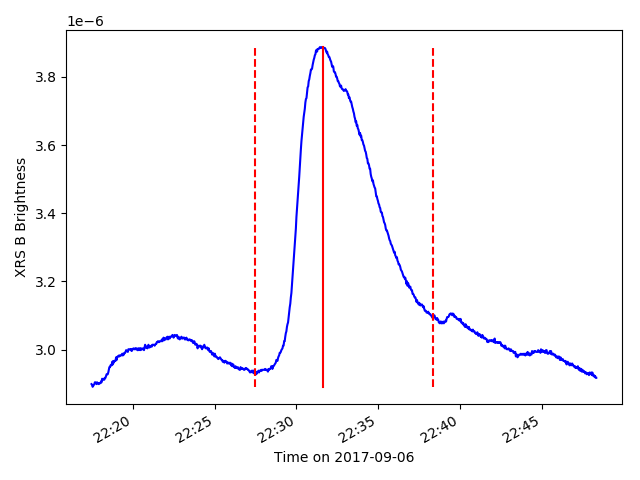
\includegraphics[scale=0.55]{flare_example.png}
    \caption{This bright flare from September 6th, 2017 shows the X-ray brightness change. The first dotted, vertical, red line indicates where the flare begins. The solid, vertical, red line indicates the peak of the flare. The final dotted, vertical, red line indicates the time the flare ends. We would like to forecast the brightness of the flare in real time, thus being able to estimate when and how bright it will peak and how when it will end and return to the brightness before the event.} 
    \label{fig:example}
\end{figure}

\section{PROBLEM STATEMENT}

For a moment in a flare, we will utilize $k$ consecutive, historical x-ray flare observations and some set of $n$ other features as our input feature vector $\vec{x} \in \mathbb{R}^{k+n}$. We will train a machine learning regressor $f:\mathbb{R}^{k+n} \to \mathbb{R}^M$ to forecast $M$ future flare x-ray brightnesses. This is the ``multi-step forecast problem". This can be done with several approaches as outlined in Section \ref{sec:approaches}. 

\section{DATA SOURCES}
Our primary event list is the \textit{Geostationary Operational Environmental Satellite} (GOES) flare catalog. We have written a Python script to retrieve this database using the SunPy API and have 90,701 flares between 1975 and 2018 \cite{sunpy}. Our main data are the GOES X-ray Sensor (XRS) observations of the Sun. Roughly every 3 seconds, GOES-XRS reports the brightness of the Sun in two x-ray passbands: a short wavelength passband from 0.5 to 4 angstroms called the A passband and a long wavelength passband from 1 to 8 angstroms called the B passband. D. We have written Python scripts that will retrieve this data using the SunPy API \cite{sunpy}. Since the median flare duration is 840 seconds and we sample roughly every 3 seconds, we have 280 GOES-XRS observations for each flare in each passband. Each flare can be divided into multiple sections of a set observation window, $k$, i.e. from observing $k$ historical data points we forecast the future. As discussed below in Section \ref{sec:approaches}, we will vary $k$ to determine an optimal length maximizing the trade-off between instantaneous predictions from only a few observations versus very accurate observations after observing most of a flare's lifetime. Thus, every moment in the flare can be associated with an observational history and future resulting in a dataset with greater than 24 million samples. 

This GOES event list is curated by hand and may miss some flares. We have obtained a larger flare list, the \textit{Reuven Ramaty High Energy Solar Spectroscopic Imager} (RHESSI) flare list that has 121,180 flares between 2002 and 2018. We can use this to augment the GOES list if we find we need more events. However, the list appears to include erroneous events. Similarly, we have obtained the flare list from Ryan et al. (2016) that identifies even more events and discriminates ``complex" flare events, when an event has multiple flares in rapid succession before returning to normal brightness \cite{ryan}. This list has 173,988 flares from 2010 to 2018. 

In addition to augmenting the event list, we can augment the feature list for each flare. Knowing information about the state of the Sun beyond merely the historical brightness of the Sun should improve our forecast. Upon talking with domain experts, we have identified a list of potentially helpful datasets and have developed an API to fetch from various sources. However, some of these datasets are only available for more recent flares, e.g. the Solar Dynamics Observatory datasets are only available from 2010 on when it was launched, hence why the more populated event lists may become helpful. This means we will have to truncate our sample list if we plan to utilize those features. 
\begin{itemize}
    \item \textbf{Solar Dynamics Observatory (SDO) Helioseismic and Magnetic Imager (HMI) magnetograms}: Flares are driven by the magnetic fields of the Sun. When the magnetic fields become complex with positive and negative polarities mixing, there is greater potential for flares. Magnetograms are images that directly allow us to estimate this mixing. We are considering using these images in a convolutional neural network to extract features or manually extracting features, e.g. the standard deviation to estimate polarity mixing around the flaring region. 
    \item \textbf{Spaceweather HMI Active Region Patch (SHARP)}: Another way to use the HMI images is to fetch the SHARP entry for the active region, active regions are regions on the Sun that are bright in EUV and have especially strong magnetic fields, that the flare belongs to. Unfortunately, our event list does not always denote the active region a flare belongs to, so we will either have to experiment with this feature on a subset of them or estimate which active region patch works best. 
    \item \textbf{Solar Radio Flux at 10.7 cm}: The solar radio flux at 10.7 is regarded as a proxy for solar activity. We have developed a Python tool that can retrieve it from the University of Colorado's Laboratory for Atmospheric and Space Physics (LASP) online archive, the LASP Interactive Solar Irradiance Datacenter. This data could be beneficial in relating the current solar activity to flaring capability and linking similar flares in the Sun's 11 year activity cycle. 
    \item \textbf{SDO Atmospheric Imaging Assembly (AIA) extreme ultraviolet (EUV) images}: Ultraviolet images reveal high-energy, complex structures on the Sun. By looking at EUV images we can also identify where filaments and other solar structures that can impact the flaring capability are. Similarly, we can refer to the Heliophysics Event Knowledgebase which provides segmentation masks for the Sun and these events. (However, these are not always reliable.) 
    \item \textbf{Large Yield Radiometer (LYRA) and Extreme Ultraviolet Variability Experiment (EVE) }: LYRA and EVE \cite{lyra} are EUV sensors that output light curves, scalar values over time, of various solar measurements. These may be helpful and have similar data to AIA's images, just in a one-dimensional time series. 
\end{itemize}

Depending on how we choose to use these lists and features, we will have dozens to hundreds of features for each of our 23+ million flare sections, corresponding to 120,000+ flares. Feature selection is one task on which we will work.

\newpage 

\section{PROPOSED APPROACHES}\label{sec:approaches}
For any given algorithm that we try, there are multiple ways to solve the multi-step forecast problem:
\begin{itemize}
    \item \textbf{One model used recursively}: This approach requires training a model to predict the immediate next time step and repeatedly employing it to create a forecast of $M$-steps. For example, with $M=2$, we could use previous observations $[y_1, y_2]$ using $f:\mathbb{R}^{k+n} \to \mathbb{R}$ to predict the immediate next step $\hat{y_3}$ and then use the same model on $[y_2, \hat{y_3}]$ to recursively predict $\hat{y_4}$ resulting in a final prediction of $[\hat{y_3}, \hat{y_4}]$,
    \item \textbf{Multiple models, one for each lag}: We train a separate many independent models for each time lag instead of reusing a single one. This is computationally more expensive but could perform better. For example, with $M=2$, we could use previous observations $[y_1, y_2]$ and predict $\hat{y_3}$ with model $f_1$ and $\hat{y_4}$ with model $f_2$ resulting in a complete prediction of $[\hat{y_3}, \hat{y_4}]$. 
    \item \textbf{One model with multiple outputs}: The previous approach does not allow models to depend on each. Instead we could train a single model $f:\mathbb{R}^{k+n}\to\mathbb{R}^M$ to outputs all the predictions. However, this will require more training data and could overfit. 
\end{itemize}
Under each of these approaches, we could use different algorithms. Thus, we will try the following learning techniques and compare their results:
\begin{enumerate}
    \item \textbf{Baseline model} - Given $k$ observations $X = [x_i, \hdots , x_{i+k}]$, we assume that the next $m$ observations is the mean of $X$. In the absence of prior work, we will use this as the simplest, baseline model. This model has high bias, and is expected to perform poorly on the test set. 
    \item \textbf{Autoregressive integrated moving average} - This is a common time series forecasting technique. It is a simple improvement on our baseline. 
    \item \textbf{Linear Regression} - We will fit a linear model to the training data. We will train the data with and without regularization and compare their accuracy on the test set. Typically, the mean square error is used as an error measure. However, since the absolute error values can vary with the intensity of the flare, we can used a more scale-dependent approach like the Mean Absolute Percentage Error (MAPE). We will also explore the effect of feature selection on the test accuracy.
    \item \textbf{Support Vector Regression(SVR)} - We will fit a kernelized support vector regressor. 
    \item \textbf{Random Forest} - We will fit a Random Forest regressor to the data. Each tree in the forest will find the locally optimal feature to split the data by minimizing an impurity measure. Feature importance can be calculated as the decrease in node impurity weighted by the probability of reaching that node. Also, we will carefully optimize hyper-parameters of number of trees and maximum tree depth. 
    \item \textbf{Long short-term memory (LSTM)} - LSTMs are a deep learning technique well-suited to time series data, as they can selectively remember important events in the past for future predictions. However, this approach will not provide any insight into feature importance, so we will implement feature selection before training the model to observe its effect on the model accuracy.
\end{enumerate}

As time allows, we will consider the following stretch goals:
\begin{itemize}
    \item Incorporating a CNN model to use raw image data.
    \item Attempting forecasting before a flare begins.
    \item Clustering flares in an unsupervised fashion.
    \item Characterizing how much concept drift may occur.
\end{itemize}

\section{PROPOSED TIME LINE AND WORK DIVISION}

Each team member will take responsibility for a different section of the project. Marcus will focus on feature extraction and selection as well as explore the benefit of online approaches. Mahesh will focus on random forest and SVR. Dave will focus on deep learning techniques. Collectively, the team will develop the simpler baseline and linear models. 

We will test and organize our code base concurrently with developing and determining optimal features for the task. Thus, throughout the project we will have approximate conclusions and will re-run experiments with a final set of features at the end.
\begin{itemize}
    \item \textbf{November 2:} Submit proposal.
    \item \textbf{November 9:} Conclude baseline and ARIMA results. Work on SHARP features.
    \item \textbf{November 16:} Have completed linear regression and SVR. Work on magnetogram features. 
    \item \textbf{November 23:} Have completed random forest architecture with easy re-run on new features. Work on 10.7 cm features. 
    \item \textbf{November 30:} Have completed LSTM model. Evaluate features theoretically and experimentally. 
    \item \textbf{December 7:} Have completed paper written for final revision and last minute work.
    \item \textbf{December 14:} Submit project write-up by 5pm.
    \item \textbf{December 15:} Prepare poster.
    \item \textbf{December 17:} Present poster describing project.
\end{itemize}

\newpage 
\section{INTERESTING SUB-PROBLEMS AND QUESTIONS}
There are many related questions that we will explore as time allows through our approaches and experiments:
\begin{itemize}
\item Are there different types of flares? In operational solar weather forecasting, flares are classified based on their peak X-ray intensity. However, this ignores all spatial structure and how they evolve. We may be able to use our database for unsupervised clustering to identify kinds of flares from a data science perspective. If we can identify these types without using the full flare observation, we may be able to add it as a feature to augment our forecast performance. Regardless of our utility, it is of scientific interest. 
\item Given X-ray observations, can we predict the EUV light curve? They are inherently related by the physics of the Sun, but the relationship can become complicated. There may be scientific conclusions if only some "types" of flares can be mapped this way. 
\item What features optimize our prediction performance? How far into the future can we reliably forecast? Conversely, what features are least important and how does that compare to the physics intuition of importance?
\item How do the various algorithms respond to the 11-year solar cycle changes? Does their performance degrade as we enter the deepest portion of solar minimum? Are flares in solar minimum different than flares in solar maximum, requiring separate regressors? 
\end{itemize}

\begin{thebibliography}{99}
\bibitem{bobra} Bobra et al., 2014, Solar Physics, 289, 3549
\bibitem{guerra} Guerra J. A., Pulkkinen A. and Uritsky V. M., 2015, Space Weather, 13, 626
\bibitem{sunpy} Hughitt et al., 2012, SunPy: Open Source Solar Data Analysis Tools for Python at \url{sunpy.org}
\bibitem{lyra} M. Dominque et al., 2013, \textit{Solar Physics}, 286, 1, 21-42 
\bibitem{nishizuka} N. Nishizuka et al., 2018, \textit{The Astrophysical Journal}, 858, 113
\bibitem{ryan} D.F. Ryan, D. F. Ryan,  M. Dominique, D. Seaton, K. Stegen and A. White, 2016, \textit{Astronomy and Astrophysics}, 592, A133
\bibitem{yu} Yu et al., 2010, Astrophysical Journal, 710, 869

\end{thebibliography}

\end{document}
